\documentclass[crop,class=article]{standalone}
%----------------------------Preamble-------------------------------%
\usepackage[dvipsnames]{xcolor}         % Color names.
\usepackage{tikz}                       % Drawing/graphing tools.
\usetikzlibrary{
    calc,                   % Calculating right angles and more.
    angles,                 % Drawing angles within triangles.
    arrows.meta,            % Latex and Stealth arrows.
    quotes,                 % Adding labels to angles.
}                                       % Libraries for tikz.
\newcommand{\MarkRightAngle}[4][.3cm]
    {\coordinate (tempa) at ($(#3)!#1!(#2)$);
     \coordinate (tempb) at ($(#3)!#1!(#4)$);
     \coordinate (tempc) at ($(tempa)!0.5!(tempb)$);%midpoint
     \draw (tempa) -- ($(#3)!2!(tempc)$) -- (tempb);}
%--------------------------Main Document----------------------------%
\begin{document}
    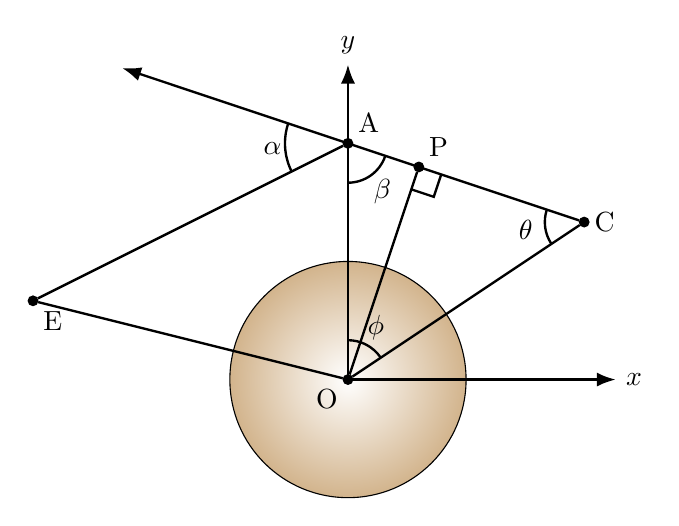
\begin{tikzpicture}[>=Latex,line width=0.3mm]
        \draw[inner color=white,outer color=Tan,thin]
            (0,0) circle (1.5);
        \begin{scope}[
            every node/.style={
                circle,
                fill=black,
                draw=black,
                inner sep=0pt,
                minimum size=3pt
            }
        ]
            \node (O) at (0,0) {};
            \node (E) at (-4,1) {};
            \node (C) at (3,2) {};
            \node (A) at (0,3) {};
            \node (P) at (0.9,2.7) {};
        \end{scope}
        \node at (O) [below left] {O};
        \node at (E) [below right] {E};
        \node at (C) [right] {C};
        \node at (A) [above right] {A};
        \node at (P) [above right] {P};
        \node (Space) at (-3,4) {};
        \draw[->] (0,0) to (0,4) node [above] {$y$};
        \draw[->] (0,0) to (3.4,0) node [right] {$x$};
        \draw (O) to (P);
        \draw (O) to (E);
        \draw (O) to (C);
        \draw (A) to (E);
        \draw[->] (C) to (Space);
        \pic[%
            "$\alpha$",
            angle eccentricity=1.2,
            angle radius=0.8cm,
            -,
            draw=black
        ]   {angle=Space--A--E};
        \pic[%
            "$\beta$",
            angle eccentricity=1.5,
            angle radius=0.5cm,
            -,
            draw=black
        ] {angle=O--A--C};
        \pic[%
            "$\theta$",
            angle eccentricity=1.5,
            angle radius=0.5cm,
            -,
            draw=black
        ]   {angle=A--C--O};
        \pic[%
            "$\phi$",
            angle eccentricity=1.5,
            angle radius=0.5cm,
            -,
            draw=black
        ]   {angle=C--O--A};
        \MarkRightAngle{O}{P}{C}
    \end{tikzpicture}
\end{document}